\documentclass[10pt]{beamer}

%%%
% PREAMBLE FOR THIS DOC 
%%%
%https://tex.stackexchange.com/questions/68821/is-it-possible-to-create-a-latex-preamble-header
\usepackage{/Users/miw267/Repos/latex_preamble/beamer_preamble}

\usetikzlibrary{matrix}


%%%
% DOCUMENT
%%%

\begin{document}

%\maketitle

%% Title page frame
%\begin{frame}
%    \titlepage 
%\end{frame}





\title{11/04/2026: Intro to Probability (Part 2)}
\author{CSCI 246: Discrete Structures}
\date{Textbook reference: Sec 31, Scheinerman}

\begin{frame}
    \titlepage 
\end{frame}


\begin{frame}
\footnotesize 
%\begin{mygreenbox}[title=Graded Quiz Pickup]
%Quizzes are in the front of the room, grouped into four bins (A-G, H-L, M-R, S-Z) by last name. The quizzes are upside down with your last name on the back. Come find yours before, during, or after class.  Only turn the quiz over if it's yours.
%\end{mygreenbox} 
%\vfill 

\begin{myredbox}[title=\text{Announcements}]

\begin{itemize}
\item I'm giving the Applied Math Seminar  tomorrow (Thursday, November 5th) at 3:10pm  in Wilson Hall \#1-144.  Title: \textit{Bayesian Multi-Sample Changepoint Inference with Linear Computational Cost.} Feel free to attend.
\item I need to cancel office hours today.  If you were planning on attending, send me an email so we can schedule an alternate time.
\end{itemize}
\end{myredbox}

\vfill 


\begin{myyellowbox}[title=Today's Agenda]
\begin{itemize}
	\item Odds and Ends: Study guide, finish slide from Monday's deck ($\approx$ 5 mins)
	\item Mini-lecture ($\approx$ 25 mins)
	\item Group exercises ($\approx$ 20 mins)
\end{itemize}


\end{myyellowbox}
\vfill 

\end{frame}





\begin{frame}{Study Guide For Quiz \#9}
\scriptsize 

\colorbox{yellow!20}{\textbf{Group exercises.}} Know how to solve the group exercises from the course meetings on Functions (10/21), Big O and Big Theta (10/28), and Algorithmic Efficiency (10/30).

\vfill 

\colorbox{red!20}{\textbf{Readings.}}   

Sec. 24 (Functions)
\vspace{-.2cm}
\begin{itemize}
\item Understand the defintion of a function, as in Examples 24.2 and 24.4.
\item Know how to prove whether function is 1-to-1 --  as in Examples 24.16 and 24.17, onto -- as in Example 24.20, or both (that is a bijection) -- as in Example 24.23.
\end{itemize}

Epp Sec 11.2 (Big-O, Big-Omega, Big-Theta Notations)
\vspace{-.2cm}
\begin{itemize}
	\item Know how to show that a function is Big-O or Big-Omega of some other function by applying the definitions of Big-O and Big-Omega, as in Example 11.2.3. 
	\item Understand the problem with Big O notation, as in Example 11.2.6.
	\item Know how to show that a function is Big-Theta of some other function by applying the definition of Big-Theta, as in Example 11.2.5a. 
	\item Know how to apply the theorem on polynomial orders, as in Example 11.2.8.
\end{itemize}

Epp Sec 11.3 (Analysis of Algorithm Efficiency I)
\vspace{-.2cm}
\begin{itemize}
\item Know how to compute the order of an algorithmic segment via computing the number of elementary operations that are performed, as in Examples 11.3.2, 11.3.3, and 11.3.4.
\item Understand the difference between worst-case, best-case, and average-case complexities, as presented in Example 11.3.1.  (For more, understand Examples 11.3.6 and 11.3.7 at a high level.)
\end{itemize}

\end{frame}



\begin{frame}[standout]
Finish slide from Monday's deck
\end{frame}

\begin{frame}[standout]
Applications \\
Of The Equally Likely Probability Formula
\end{frame}


\begin{frame}
\begin{mygreenbox}[title=\text{Reminder of Proposition: Equally Likely Probability Formula}]
If $(P,S)$ is a probability space in which all outcomes are equally likely and E is an event in $S$, then the probability of $E$ is
%
\begin{align*}
P(E) = \frac{|E|}{|S|} = \frac{\text{the number of outcomes in } E }{\text{the number of outcomes in } S}	
\end{align*}
\end{mygreenbox}
\end{frame}



\begin{frame}
\begin{mybluebox}[title=\text{Example: Ten Dice}]
Ten dice are tossed.  What is the probability of getting the same number on all the die? \\

\only<2>{\alert{What is the sample space?}}%
\onslide<3->
Let $S$ be the sample space.  That is,
\begin{align*}
 S&=\bigg\{(\texttt{1,1,1,1,1,1,1,1,1,1,1}), (\texttt{1,1,1,1,1,1,1,1,1,2}), \hdots,  \\
 & \qquad \qquad (\texttt{6,6,6,6,6,6,6,6,6,6,6,6})\bigg\}
\end{align*}
%
\onslide<4->
Let $E \subset S$ be the event that all of the the die show the same number.
\only<5>{\alert{Are all outcomes equally likely?}}%
\onslide<6->
Then by the equally likely probability formula,
\begin{align*}
P(E) = 	\frac{|E|}{|S|}
\end{align*}
\only<7>{\alert{What are $|E|$ and $|S|$?}}%
\onslide<8->
Now $|S|=6^{10}$ and $|E|=6$.
\onslide<9->
Hence,
%
\begin{align*}
P(E) = 	\frac{|E|}{|S|} = \frac{6}{6^{10}} = \bigg(\frac{1}{6}\bigg)^{9} \approx \frac{1}{10 \; \text{million}.}
\end{align*}
\end{mybluebox}

\end{frame}






\begin{frame}
\begin{mybluebox}[title=\text{Example: Coin tossing}]
A coin is tossed five times.  What is the probability that we see exactly two heads?  \\

\only<2>{\alert{What is the sample space?}}%
\onslide<3->
Let $S$ be the sample space.  That is,
 \[ S=\bigg\{\texttt{(H,H,H,H,H)}, \texttt{(H,H,H,H,T)}, \hdots, \texttt{(T,T,T,T,T)} \bigg\}. \]
\onslide<4->
Let $E \subset S$ be the event that exactly two heads are observed.
\only<5>{\alert{Are all outcomes equally likely?}}%
\onslide<6->
Then by the equally likely probability formula,
\begin{align*}
P(E) = 	\frac{|E|}{|S|}
\end{align*}
\only<7>{\alert{What are $|E|$ and $|S|$?}}%
\onslide<8->
Now $|S|=2^{5}$ and $|E|=\binom{5}{2}$.
\onslide<9->
Hence,
%
\begin{align*}
P(E) = 	\frac{|E|}{|S|} = \frac{\binom{5}{2}}{2^{5}} = \frac{10}{32} \approx 0.3125.
\end{align*}
\end{mybluebox}

\end{frame}

\begin{frame}
\small 
\begin{mybluebox}[title=\text{Example: Four of a kind}]
A poker hand is called a \textit{four of a kind} if four of the five cards show the same value (e.g. all 7s or all kings).  What is the probability that a poker hand is a four of a kind?  \\

\only<2>{\alert{What is the sample space?}}%
\onslide<3->
Let $S$ be the sample space.  That is,
\[S=\bigg\{ \set{A\spadesuit 2 \spadesuit 3 \spadesuit 4 \spadesuit 5 \spadesuit}, \;   \hdots, \; \set{9 \heartsuit 10 \heartsuit J \heartsuit Q \heartsuit K \heartsuit} \bigg\}. \]
\onslide<4->
Let $E \subset S$ be the event that the poker hand is a four of a kind.
\only<5>{\alert{Are all outcomes equally likely?}}%
\onslide<6->
Then by the equally likely probability formula,
\begin{align*}
P(E) = 	\frac{|E|}{|S|}
\end{align*}
\only<7>{\alert{What are $|E|$ and $|S|$?}}%
\onslide<8->
Now $|S|=\binom{52}{5}$ and $|E|=13 \times 48$.
\onslide<9->
Hence,
%
\begin{align*}
P(E) = 	\frac{|E|}{|S|} = \frac{13 \times 48}{\binom{52}{5}} \approx 0.00024.
\end{align*}
\vfill
\textbf{Final Answer}: The probability of getting a four of a kind in a 5-card poker hand is approximately 0.00024, or about 1 in 4,167 hands.
\end{mybluebox}

\end{frame}


\begin{frame}[standout]
Probability of Complements
\end{frame}


\begin{frame}
\begin{mybluebox}[title=\text{The Birthday Problem}]
What is the probability that at least two people in this room share a birthday?
\end{mybluebox}
\vfill 
\onslide<2->{\colorbox{red!30}{\textbf{Hint.}} To solve problems like this, it can be helpful to use the probability of a complement.} \onslide<3>{\alert{What is that?}}
\vfill 
\only<4-6>{
\begin{mygreenbox}[title=\text{A Few Basic Properties of Probability}]
Let $(S,P)$ be a probability space. Then
\begin{itemize}
	\item<4-6>[(a)] (Probability of entire space.) $P(S)=1$. 
	\item<5-6>[(b)] (Probability of empty set.)  $P(\emptyset)=0$. 
	\item<6-6>[(c)] \alert<6->{(Probability of complement.) $P(\overline{A}) = 1-P(A)$,} \\
		\alert<6-6>{where $\overline{A} \defeq S-A$ is called the \textit{complement} of $A$ (i.e. A \underline{didn't} happen).}
\end{itemize}
\end{mygreenbox}
}
\onslide<7->{
\colorbox{green!30}{\textbf{Solution.}}
Let $A$ be the event that at least two people in this room share a birthday.   It’s easier to work with the event $\overline{A}$ (that \textit{everyone's birthday is different}).  Suppose there are 25 people in this room. Then 
 \[ P(A) = 1- P(\overline{A}) = 1 - \frac{(365 \cdot 364 \cdots 341)}{365^{25}} \approx 0.57 \]
}
\end{frame}


%\begin{frame}
%\begin{mybluebox}[title=\text{Example: The Gambler's Puzzle (de Méré, 1654)}]
%Which bet is more likely to win? 
%\begin{itemize}
%\item[(a)] At least one 6 in 4 rolls of a die.
%\item[(b)] At least one double-six in 24 rolls of a pair of dice.
%\end{itemize}
%\end{mybluebox}
%\vfill 
%\onslide<2->{\colorbox{green!30}{\textbf{Hint.}} To solve problems like this, it can be helpful to use the probability of a complement.} \onslide<3->{\alert{What is that?}}
%\vfill 
%\onslide<4->{
%\begin{mygreenbox}[title=\text{A Few Basic Properties of Probability}]
%Let $(S,P)$ be a probability space. Then
%\begin{itemize}
%	\item<4->[(a)] (Probability of entire space.) $P(S)=1$. 
%	\item<5->[(b)] (Probability of empty set.)  $P(\emptyset)=0$. 
%	\item<6->[(c)] \alert<6->{(Probability of complement.) $P(\overline{A}) = 1-P(A)$,} \\
%		\alert<6->{where $\overline{A} \defeq S-A$ is called the \textit{complement} of $A$ (i.e. A \underline{didn't} happen).}
%\end{itemize}
%\end{mygreenbox}
%}
%\end{frame}


\begin{frame}
\small
\begin{mybluebox}[title=\text{Example: The Gambler's Puzzle (de Méré, 1654)}]
Which bet is more likely to win? 
\begin{itemize}
\item[(a)] At least one 6 in 4 rolls of a die.
\item[(b)] At least one double-six in 24 rolls of a pair of dice.
\end{itemize}

\onslide<2->
\textbf{Bet (a).}
\only<2>{\alert{What is the sample space?}}%
\onslide<3->
Let $S$ be the sample space.  That is,
\[ S=\set{(\texttt{1,1,1,1}), (\texttt{1,1,1,2}), \hdots, (\texttt{6,6,6,6})} \]
\onslide<4->
Let $E \subset S$ be the event that at least one die shows a 6.  Its complement is
\[ \overline{E} = \set{(\texttt{1,1,1,1}), (\texttt{1,1,1,2}), \hdots, (\texttt{5,5,5,5})} \]
\only<5>{\alert{What are $|\overline{E}|$ and $|S|$?}}%
\onslide<6->
Now $|S|=6^{4}$ and $|\overline{E}|=5^{4}$.
\only<7>{\alert{Are all outcomes equally likely?}}%
\onslide<8->
Hence, by the complement property and the equally likely probability formula,
\begin{align*}
P(E) = 1 - P(\overline{E}) = 1 - \frac{|\overline{E}|}{|S|} = 1 - \bigg(\frac{5}{6}\bigg)^{4} \approx 0.518.
\end{align*}
\end{mybluebox}
\end{frame}


\begin{frame}
\small
\begin{mybluebox}[title=\text{Example: The Gambler's Puzzle (de Méré, 1654), continued}]
\textbf{Bet (b).}
\only<1>{\alert{What is the sample space?}}%
\onslide<2->
Let $S$ be the sample space.  Each roll is a pair, so an outcome is a list of 24 pairs:
\[ S=\set{\big((\texttt{1,1}), \hdots, (\texttt{1,1})\big), \;  \big((\texttt{1,1}), \hdots, (\texttt{1,2})\big), \; \hdots, \; \big((\texttt{6,6}), \hdots, (\texttt{6,6})\big)} \]
\onslide<3->
Let $E \subset S$ be the event that at least one roll is $(\texttt{6,6})$.  Its complement is the set of lists in which every roll is one of the other 35 pairs:
\[ \overline{E}=\set{\big((\texttt{1,1}), \hdots, (\texttt{1,1})\big), \;  \big((\texttt{1,1}), \hdots, (\texttt{1,2})\big), \; \hdots, \; \big((\texttt{6,5}), \hdots, (\texttt{6,5})\big)} \]

\only<4>{\alert{What are $|\overline{E}|$ and $|S|$?}}%
\onslide<5->
Now $|S|=36^{24}$ and $|\overline{E}|=35^{24}$.
\only<6>{\alert{Are all outcomes equally likely?}}%
\onslide<7->
Hence, by the complement property and the equally likely probability formula,
\begin{align*}
P(E) = 1 - P(\overline{E}) = 1 - \frac{|\overline{E}|}{|S|} = 1 - \bigg(\frac{35}{36}\bigg)^{24} \approx 0.491.
\end{align*}
\onslide<8->
\textbf{Answer.} Bet (a) wins more often than it loses; bet (b) loses more often than it wins.
\end{mybluebox}
\end{frame}





\begin{frame}[standout]
Warning: \\
Outcomes Aren't Always Equally Likely
\end{frame}


\begin{frame}
\begin{myredbox}[title=Question]
Two dice are rolled.  What is $P(\text{sum} = 7)$?
\end{myredbox}
\vfill
\begin{columns}[T,onlytextwidth]
\begin{column}{0.55\textwidth}

\only<2->{\textbf{Warning:} This is a trap for \qq{Equally Likely} thinking!}

\begin{itemize}
\item<3-> \textbf{The trap:} \qq{There are 11 possible sums, so $\frac{1}{11}$.}
\item<4-> \textbf{Answer:} $\frac{6}{36} = \frac{1}{6}$.  The 36 ordered pairs are equally likely; the 11 sums are not.
\item<5-> \textbf{Catan players know this:} the 6 and 8 tiles are the valuable ones.
\end{itemize}
\end{column}
\begin{column}{0.4\textwidth}
\onslide<5->{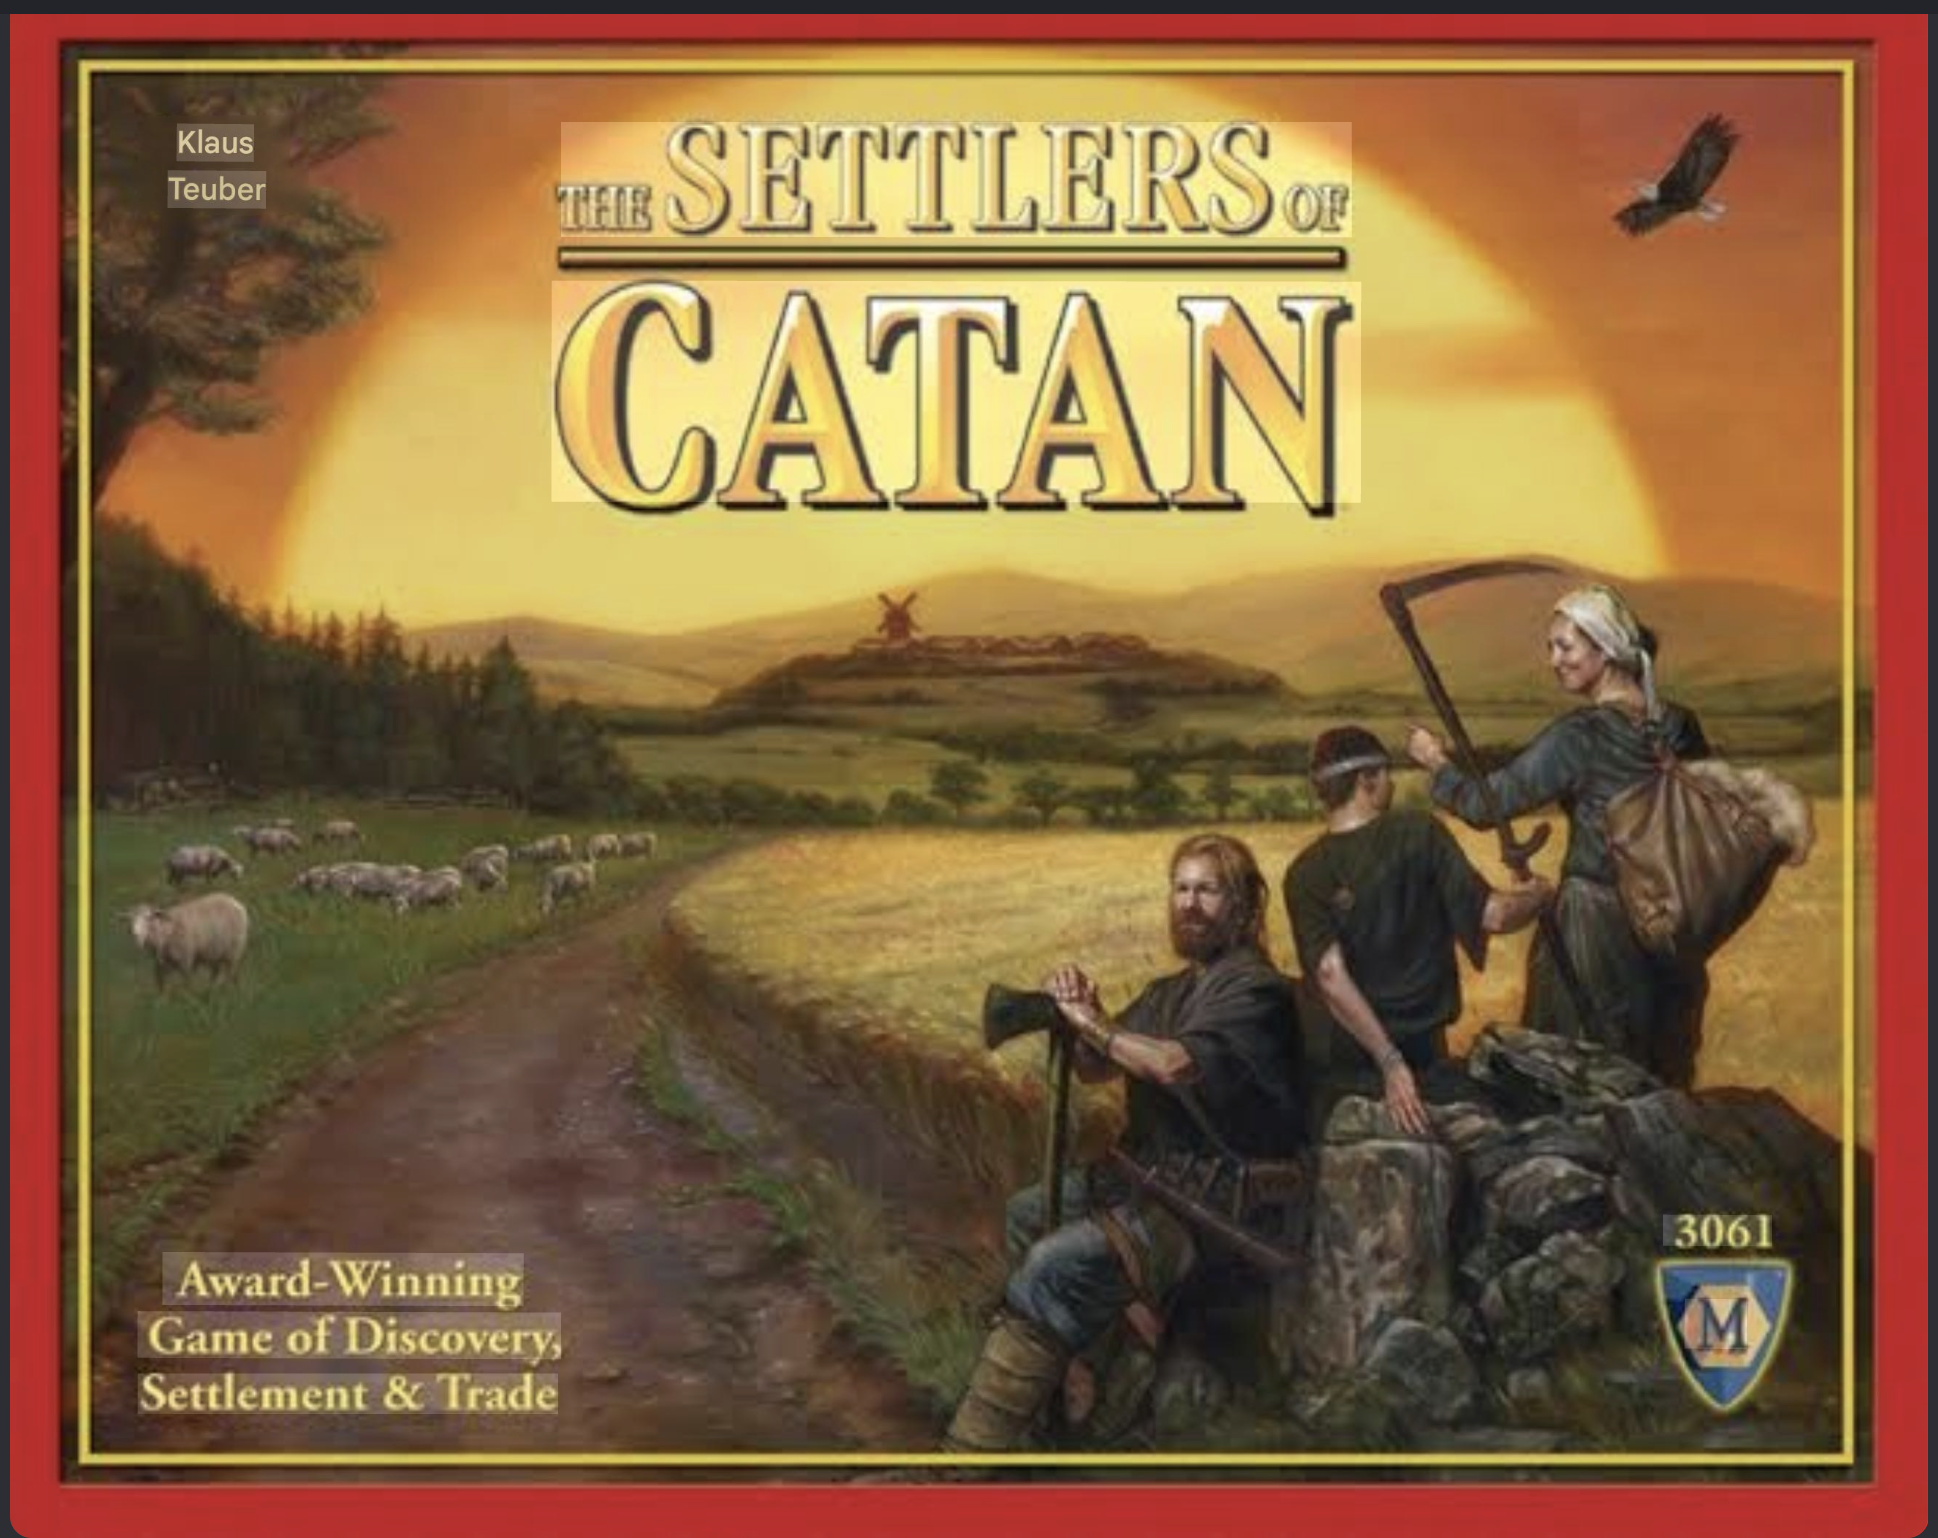
\includegraphics[width=\textwidth]{images/catan}}
\end{column}
\end{columns}
\vfill
\end{frame}

\begin{frame}

\begin{myredbox}[title=\text{Warning: Outcomes Aren't Always Equally Likely}]
Consider the probability space $(S,P)$ where the sample space
\[ S=\set{A,B,C,D,F}\]
is your possible grades in CSCI 246. Suppose that you have been performing well in the class so far, and the probability of you obtaining each grade is given by
\[ P(A)= .50, \; P(B)= .30, \;  P(C)= .10, \;  P(D)= .07, \;  P(F)= .03 \]
\pause 
Suppose $U=\set{D,F}$ is the event that you get a grade that you might consider \underline{unsatisfactory}.
Then
\[ P(U) = \sum_{s \in U} P(s) = P(D) + P(F) = .07 + .03 = .10\]
\pause 
Here, the equally likely probability formula gives the \alert{wrong} result:
\[ P(E) \neq \frac{|E|}{|S|} = \frac{2}{5} = .40\]
\end{myredbox}

\end{frame}







\begin{frame}[standout]
General addition rule
\end{frame}

%\begin{frame}
%
%\begin{myyellowbox}[title=\text{Practice Reading Quiz (Events)}]
%Let $A$ and $B$ be events in a probability space $(S,P)$.  
%
%\begin{enumerate}
%\item State whether the equation below is true or false:
%\[ P(A \cup B) = P(A) + P(B) \]	
%\item If the equation is true, provide a proof.  If the equation is false, provide the correct equation.
%\end{enumerate}
%
%\end{myyellowbox}
%	
%\end{frame}
%



\begin{frame}
\scriptsize 
\begin{mygreenbox}[title=\text{Proposition: Basic Properties of Probability}]
Let $(S,P)$ be a probability space. Then
\begin{itemize}
	\item[(a)] (Probability of entire space.) $P(S)=1$. 
	\item[(b)] (Probability of empty set.)  $P(\emptyset)=0$. 
	\item[(c)] (Probability of complement.) $P(\overline{A}) = 1-P(A)$, \\
		where $\overline{A} \defeq S-A$ is called the \textit{complement} of $A$ (i.e. A \underline{didn't} happen).
	\item[(d)]  (General addition rule.)  $P(A \cup B) = P(A) + P(B) - P(A \cap B)$, \\
	where $A$ and $B$ be events.
\end{itemize}
\end{mygreenbox}

\pause 
\vfill 
\begin{myredbox}[title=\text{Remark: General Addition Rule As Inclusion-Exclusion}]
Recall the inclusion-exclusion formula (with two sets):
\[ |A \cup B| = |A| + |B| - |A \cap B|\]
The general addition rule is this same formula, but where we measure size using probabilities $P(\cdot)$ instead of cardinality $|\cdot|$.
\end{myredbox}

\pause 
\vfill 
\begin{myyellowbox}[title=\text{Additional properties}]
As a consequence of the  general addition rule, we also have
\begin{itemize}
	\item[(e)] (Subadditivity.) $P(A \cup B) \leq P(A) + P(B)$. 
	\item[(f)] (Additivity.) If $A \cap B = \emptyset$, then  $P(A \cup B) = P(A) + P(B)$.
\end{itemize}
\end{myyellowbox}

\end{frame}


\begin{frame}
\footnotesize 
\begin{mygreenbox}[title=\text{Example: Drawing a Card from a Deck}]
You draw a single card from a standard 52-card deck. What is the probability that the card is either a heart or a face card? \\
\\
\pause 
Let
\begin{itemize}
\item A = the event that the card is a \textbf{heart} $\rightarrow P(A) = 1/4$.\\
\item B = the event that the card is a \textbf{face card} (Jack, Queen, or King of any suit) $\rightarrow P(B) = 3/13$. 
\end{itemize}

\pause 
Note that some cards belong to \textbf{both} events: the \textbf{face cards that are also hearts} (Jack, Queen, and King of hearts). \\


The overlap $A \cap B$ satisfies
\[P(A \cap B)  = \frac{3}{52}.\]

\pause 
To find $P(A \cup B)$, we use the \textbf{general addition rule}.
%
\begin{align*}
P(A \cup B) &= P(A) + P(B) - P(A \cap B) \\
&= \frac{1}{4} + \frac{3}{13} - \frac{3}{52} \\
&= \frac{11}{26} \approx 0.42
\end{align*}
 	
\pause 
\textbf{Final answer.} The probability of drawing either a heart or a face card is $\frac{11}{26}$, which is \textbf{less than} the sum of the individual probabilities because we subtract the overlap.
\end{mygreenbox}

	
\end{frame}




\begin{frame}[standout]
Group exercises
\end{frame}

\begin{frame}{Random Group Assignments}
%%% TABLE 1: by last name
\begin{columns}
\begin{column}{0.33\textwidth}
Ashley, Isabelle: 3 \\ 
Bailey, Tanna: 7 \\ 
Blaisdell, Olyver: 11 \\ 
Brown, Ashton: 5 \\ 
Cardenas, Dominic: 6 \\ 
Cutler, George: 9 \\ 
Fabik, Roland: 10 \\ 
Fellows, Audrey: 6 \\ 
Fitzgerald, Ryan: 8 \\ 
Fuller, Ryan: 2 \\ 
Griffen, Clara: 7 \\ 
Grutsch, Tanner: 6 \\\end{column}
\begin{column}{0.33\textwidth}
Hager, Nathan: 10 \\ 
Horner, Jayden: 11 \\ 
Johnson, Jaret: 1 \\ 
Kintzel, Samantha: 10 \\ 
Lameres, Alexis: 2 \\ 
Lee, Holden: 1 \\ 
Mayala, Reece: 3 \\ 
McLean, Connor: 3 \\ 
Mcbride, Daniel: 9 \\ 
Miller, Maverick: 9 \\ 
Moss, Emily: 12 \\ 
Mousseau, Matthew: 12 \\\end{column}
\begin{column}{0.33\textwidth}
Neuman, Evan: 4 \\ 
Putnam, John: 1 \\ 
Ramos, Vydel: 5 \\ 
Rathbun, Jedidiah: 4 \\ 
Roberts, Matthew: 8 \\ 
Roller, Nathan: 12 \\ 
Ryan, Otis: 8 \\ 
Shevtsov, Timothy: 11 \\ 
Stensland, Emma: 7 \\ 
Thiessen, Logan: 4 \\ 
Thompson, Jaiden: 2 \\ 
Vath, Ethan: 5 \\\end{column}
\end{columns}
\end{frame}


\begin{frame}{Group exercises}
\small
\begin{enumerate} \small
	\item (More poker hands.) Give the probability of obtaining the various hands below in a game of 5-card poker.
	\begin{itemize}	 \footnotesize 
	\item[a.] A \textbf{three of a kind}. This means three cards of the same rank and two other cards of different ranks, such as three 10s, a 7, and a jack.
	\item[b.] A \textbf{full house.} This is three cards with one common rank and two other cards of another common rank, such as three queens and two 4s.
	\item[c.] A \textbf{single pair.} This is two cards with the same rank and three other cards with three other ranks, such as two 9s, a king, an 8, and a 5.
	\item[d.] \textbf{Two pairs.} This is two cards with one common rank, two more cards with another common rank, and the remaining card has yet another rank, such as two jacks, two 8s, and a 3.
	\item[e.] A \textbf{flush.}  This means all five cards have the same suit.
	\end{itemize}
	\item Prove Scheinerman Proposition 31.8.   You may assume the the general addition rule (Scheinerman Proposition 31.7) holds.
	\item Three dice are rolled.  What is the probability that... (a) ... none of the dice shows 1? (b)... at least one die shows 1? (c) ... at least one die shows 2? (d) ... none of the dice shows 1 or 2? (e) ... at least one die shows 1 or at least one die shows 2 (or both)? (f) .... at least one die shows 1 and at least one die shows 2?
\end{enumerate}

\end{frame}


\begin{frame}{Solution to Group Exercise \#1a}
\footnotesize 
 \colorbox{blue!30}{\textbf{Problem.}} What is the probability of getting a \textbf{three of a kind} in a 5-card poker hand? 
 \vfill 

 \colorbox{green!30}{\textbf{Solution.}} Let $S$ be the sample space.  That is, 
\[S=\bigg\{ \set{A\spadesuit 2 \spadesuit 3 \spadesuit 4 \spadesuit 5 \spadesuit}, \;   \hdots, \; \set{9 \heartsuit 10 \heartsuit J \heartsuit Q \heartsuit K \heartsuit} \bigg\}. \]
Let $E \subset S$ be the event that the poker hand is a three of a kind. Then by the equally likely probability formula, 
\begin{align*}
P(E) = 	\frac{|E|}{|S|} = \frac{\text{\# of three of a kind poker hands}}{\text{\# of poker hands}}
\end{align*}
Now $|S|=\binom{52}{5} =  2,598,960$, so we just need to find $|E|$.  We proceed in steps:

\begin{enumerate} \footnotesize 
\item \textbf{Choose the rank} for the three matching cards 	(e.g., three Kings or three 7s).  There are 13 possible ranks.
\item \textbf{Select 3 of the 4 suits} for that rank:  $\binom{4}{3}=4$.
\item  \textbf{Choose two kicker cards} (the remaining two cards that don't match the three of a kind rank). 
	\begin{itemize} \footnotesize 
	\item[a.] 	\textbf{Choose 2 different ranks} from the remaining 12 ranks: $\binom{12}{2} = 66$ 
	\item[b.] \textbf{Select 1 suit} for each chosen rank: $\binom{4}{1} \times \binom{4}{1} = 16$
	\end{itemize}
\item \textbf{Combine the choices}:  $|E|=13 \times 4 \times 66 \times 16 = 54,912$.
\end{enumerate}
\vspace{-.1cm}
\alert{\textbf{Final Answer.}} The probability of getting a three of a kind in a 5-card poker hand is $\frac{54,912}{2,598,960} \approx 0.021128$, or about 1 in 47 hands.
\end{frame}

\begin{frame}{Solution to Group Exercise \#1b}
\footnotesize 
 \colorbox{blue!30}{\textbf{Problem.}} What is the probability of getting a \textbf{full house} in a 5-card poker hand? 
\vfill 

 \colorbox{green!30}{\textbf{Solution.}} Let $S$ be the sample space.  That is, 
\[S=\bigg\{ \set{A\spadesuit 2 \spadesuit 3 \spadesuit 4 \spadesuit 5 \spadesuit}, \;   \hdots, \; \set{9 \heartsuit 10 \heartsuit J \heartsuit Q \heartsuit K \heartsuit} \bigg\}. \]
Let $E \subset S$ be the event that the poker hand is a full house. Then by the equally likely probability formula, 
\begin{align*}
P(E) = 	\frac{|E|}{|S|} = \frac{\text{\# of full house poker hands}}{\text{\# of poker hands}}
\end{align*}
Now $|S|=\binom{52}{5} =  2,598,960$, so we just need to find $|E|$.   We proceed in steps:

\begin{enumerate} \footnotesize 
\item \textbf{Choose the rank} for the three matching cards 	(e.g., three Kings or three 7s).  There are 13 possible ranks.
\item \textbf{Select 3 of the 4 suits} for that rank:  $\binom{4}{3}=4$.
\item \textbf{Choose the rank} for the two matching cards 	(e.g., two Queens or two 6s).  There are 12 possible ranks which differ from the three-of-a-kind rank.
\item \textbf{Select 2 of the 4 suits} for that rank:  $\binom{4}{2}=6$.
\item \textbf{Combine the choices}:  $|E|=13 \times 4 \times 12 \times 6 = 3,744$.
\end{enumerate}

\alert{\textbf{Final Answer.}} The probability of getting a three of a kind in a 5-card poker hand is $\frac{3,744}{2,598,960} \approx 0.00144$, or about 1 in 694 hands.
\end{frame}

\begin{frame}{Solution to Group Exercise \#1c}
\footnotesize 
 \colorbox{blue!30}{\textbf{Problem.}} What is the probability of getting a \textbf{single pair} in a 5-card poker hand?
\vfill 

 \colorbox{green!30}{\textbf{Solution.}} Let $S$ be the sample space.  That is, 
\[S=\bigg\{ \set{A\spadesuit 2 \spadesuit 3 \spadesuit 4 \spadesuit 5 \spadesuit}, \;   \hdots, \; \set{9 \heartsuit 10 \heartsuit J \heartsuit Q \heartsuit K \heartsuit} \bigg\}. \]
Let $E \subset S$ be the event that the poker hand is a single pair. Then by the equally likely probability formula, 
\begin{align*}
P(E) = 	\frac{|E|}{|S|} = \frac{\text{\# of single pair poker hands}}{\text{\# of poker hands}}
\end{align*}
Now $|S|=\binom{52}{5} =  2,598,960$, so we just need to find $|E|$.  We proceed in steps:

\begin{enumerate} \footnotesize 
\item \textbf{Choose the rank} for the two matching cards 	(e.g., two Kings or two 7s).  There are 13 possible ranks.
\item \textbf{Select 2 of the 4 suits} for that rank:  $\binom{4}{2}=6$.
\item  \textbf{Select 3 other ranks} for the remaining 3 cards (out of the 12 ranks which differ from the single pair rank): $\binom{12}{3}=220$. 
\item \textbf{Select 1 suit for each of the 3 different ranks}: $\binom{4}{1} \times \binom{4}{1} \times \binom{4}{1} = 64.$
\item \textbf{Combine the choices}:  $|E|=13 \times 6 \times 220 \times 64 = 1,098,240$.
\end{enumerate}
\vspace{-.1cm}
\alert{\textbf{Final Answer.}} The probability of getting a single pair in a 5-card poker hand is $\frac{1,098,240}{2,598,960} \approx 0.42257$, or about 1 in 2.37 hands.
\end{frame}



\begin{frame}{Solution to Group Exercise \#1d}
\footnotesize 
 \colorbox{blue!30}{\textbf{Problem.}} What is the probability of getting \textbf{two pairs} in a 5-card poker hand?
\vfill 

 \colorbox{green!30}{\textbf{Solution.}} Let $S$ be the sample space of poker hands. 
 % That is, 
%\[S=\bigg\{ \set{A\spadesuit 2 \spadesuit 3 \spadesuit 4 \spadesuit 5 \spadesuit}, \;   \hdots, \; \set{9 \heartsuit 10 \heartsuit J \heartsuit Q \heartsuit K \heartsuit} \bigg\}. \]
Let $E \subset S$ be the event that the poker hand is two pairs. Then by the equally likely probability formula, 
\begin{align*}
P(E) = 	\frac{|E|}{|S|} = \frac{\text{\# of two pair poker hands}}{\text{\# of poker hands}}
\end{align*}
Now $|S|=\binom{52}{5} =  2,598,960$, so we just need to find $|E|$.  We proceed in steps:

\begin{enumerate} \footnotesize 
\item \textbf{Choose ranks} for the pairs (e.g., we might have a pair of Kings and pair of 7s):  $\binom{13}{2}=78$.
\item \textbf{Select 2 of the 4 suits} for each of those ranks:  $\binom{4}{2} \binom{4}{2}=6 \times 6$.
\item \textbf{Choose the rank} for the fifth card.  There are $\binom{11}{1}=11$ ranks which differ from those of the two pairs.
\item \textbf{Select 1 of the 4 suits} for that rank:  $\binom{4}{1}=4$.
\item \textbf{Combine the choices}:  $|E|=78 \times 6  \times 6 \times 11 \times 4 = 123,552$.
\end{enumerate}
\vspace{-.1cm}
\alert{\textbf{Final Answer.}} The probability of getting two pairs in a 5-card poker hand is $\frac{123,552}{2,598,960} \approx 0.0475$, or about 1 in 21 hands.
\end{frame}

\begin{frame}{Solution to Group Exercise \#1e}
\footnotesize 
 \colorbox{blue!30}{\textbf{Problem.}} What is the probability of getting a \textbf{flush} in a 5-card poker hand?
\vfill 
 \colorbox{red!30}{\textbf{Remark.}} A \textbf{flush} consists of five cards of the \textit{same suit}, but \textit{not in sequential order}. For example: $2\spadesuit 5\spadesuit 8\spadesuit J\spadesuit Q\spadesuit$.  If the cards are in sequence, it would be a \textbf{straight flush} instead.  
 
\vfill 

 \colorbox{green!30}{\textbf{Solution.}} Let $S$ be the sample space of poker hands.  
 %That is, 
%\[S=\bigg\{ \set{A\spadesuit 2 \spadesuit 3 \spadesuit 4 \spadesuit 5 \spadesuit}, \;   \hdots, \; \set{9 \heartsuit 10 \heartsuit J \heartsuit Q \heartsuit K \heartsuit} \bigg\}. \]
Let $E \subset S$ be the event that the poker hand is a flush.  We write $E=A-B$, where $A$ is the number of flushes (including straight flushes), and $B$ is the number of straight flushes.  Hence, $|E| = |A|-|B|$. 
%Then by the equally likely probability formula, $P(E) = 	\frac{|E|}{|S|} $. 



\begin{minipage}[t]{0.45\textwidth}
\scriptsize 
To find $|A|$:
\begin{enumerate}
\item \textbf{Choose the suit}: There are 4 suits.  
\item \textbf{Select 5 cards from the suit}: $ \binom{13}{5} = 1,287$.
\item \textbf{Combine the choices}: $|A| = 4 \times 1287 = 5,148$.
\end{enumerate}
\end{minipage} %
\hfill
\begin{minipage}[t]{0.45\textwidth}
\scriptsize 
To find $|B|$:
\begin{enumerate} 
\item \textbf{Choose the suit}: There are 4  suits.  
\item \textbf{Select the straight flush in the suit}: For each suit, there are 10 straight flushes, (from $A-2-3-4-5$ to $10-J-Q-K-A$).
\item \textbf{Combine the choices}: $|B| = 4 \times 10 = 40$.
\end{enumerate}
\end{minipage}

\footnotesize
Hence, the number of valid flush hands is  $ |E| = |A|-|B| = 5,148 - 40 = 5,108$.

\vspace{-.1cm}
\alert{\textbf{Final Answer.}} The probability of getting a flush is $\frac{5,108}{2,598,960} \approx 0.001965$, or about 1 in 509 hands.
\end{frame}



\begin{frame}{Solution to Group Exercise \#2}
\scriptsize  
 \colorbox{blue!30}{\textbf{Problem.}} A Let $(S,P)$ be a probability space. Then
\begin{itemize}
	\item[(a)] (Probability of entire space.) $P(S)=1$. 
	\item[(b)] (Probability of empty set.)  $P(\emptyset)=0$. 
	\item[(c)] (Probability of complement.) $P(\overline{A}) = 1-P(A)$, \\
		where $\overline{A} \defeq S-A$ is called the \textit{complement} of $A$ (i.e. A \underline{didn't} happen).
	\item[(d)]  (General addition rule.)  $P(A \cup B) = P(A) + P(B) - P(A \cap B)$, \\
	where $A$ and $B$ be events.
	\item[(e)] (Subadditivity.) $P(A \cup B) \leq P(A) + P(B)$. 
	\item[(f)] (Additivity.) If $A \cap B = \emptyset$, then  $P(A \cup B) = P(A) + P(B)$.
\end{itemize}
Assume (d) above and prove the rest.

 \vfill
  \colorbox{green!30}{\textbf{Solution.}}
 \begin{itemize}
	\item[(a)]  By the defs. of probability space and event, $P(S)= \sum_{s \in S} P(s) = 1.$ 
	\item[(b)]  By the defs. of probability space and event,  $P(\emptyset)=0 = \sum_{s \in \emptyset} P(s) = 0$. 
	\item[(c)] Using the general addition rule with $B=\overline{A}$:
	%
	\begin{align*}
	P(A \cup \overline{A}) &= P(A) + P(\overline{A}) - P(A \cap \overline{A}) \\
	\implies P(S) &= P(A) + P(\overline{A}) - P(\emptyset) \\
	\implies 1 &= P(A) + P(\overline{A}) - 0 && \scripttext{by (a), (b)}
	\end{align*}
	%
	Algebra gives the result.
	\item[(e)] This holds by the general addition rule, noting that $P(A \cap B) \geq 0$.
	\item[(f)] If $A \cap B = \emptyset$, then $P(A \cap B) =0$ by part (b).  Hence, the result follows by the general addition rule.
\end{itemize}

\end{frame}

\begin{frame}{Solution to Group Exercise \#3}
\scriptsize 
 \colorbox{blue!30}{\textbf{Problem.}} Three dice are rolled.  What is the probability that...
    \begin{columnsonlytextwidth}
    \begin{column}{0.35\textwidth}
        \begin{itemize} \tiny 
		\item[a.)] ... none of the dice shows 1? 
		\item[b.)] ... at least one die shows 1? 
		\item[c.)] ... at least one die shows 2?
        \end{itemize}
    \end{column}
    \begin{column}{0.55\textwidth}
        \begin{itemize}  \tiny 
		\item[d.)] ... none of the dice shows 1 or 2?
		\item[e.)]  ... at least one die shows 1 or at least one die shows 2 (or both)? 
		\item[f.)] .... at least one die shows 1 and at least one die shows 2?
        \end{itemize}
    \end{column}
    \end{columnsonlytextwidth}
 \vfill 
  \colorbox{green!30}{\textbf{Solution.}}  
\begin{align*}
\text{Define the following events} &&  A &= \text{at least one die shows 1} &\quad  B &= \text{at least one die shows 2} \\
 \text{So the complementary events are}&&  \overline{A} &= \text{none of the dice show 1} &\quad   \overline{B} &= \text{none of the dice show 2}
\end{align*}
%
\vspace{-.5cm}
 \begin{itemize}
\item[a.)]  The outcomes in event $\overline{A}$ are the lists of length 3 with outcomes chosen from the set $\set{2,3,4,5,6}$.  Hence $|A| = 5^3$. By the equally likely probability formula,  $P(\overline{A}) = \frac{|A|}{|S|} = \frac{5^3}{6^3} \approx  0.5787$.   
\item[b.)] By the probability of a complementary event, $P(A) =  1- P(\overline{A}) \approx 1-0.5787 = 0.4213$. 
\item[c.)] $P(B) = P(A) \approx 0.4213$.
\item[d.)] The outcomes in event $\overline{A} \cap \overline{B}$ are the lists of length 3 with outcomes chosen from the set $\set{3,4,5,6}$.   Hence $|\overline{A} \cap \overline{B}| = 4^3$. By the equally likely probability formula,  $P(\overline{A} \cap \overline{B}) = \frac{|\overline{A} \cap \overline{B}|}{|S|} = \frac{4^3}{6^3} \approx  0.2962$. 
\item[e.)] By the probability of a complementary event, $P(A \cup B) =  1- P(\overline{A \cup B})$.   By DeMorgan's laws for sets (or intuition), $\overline{A \cup B}  = \overline{A} \cap \overline{B}$. Hence, using part (d), $P(\overline{A \cup B}) = 0.2962$, and so $P(A \cup B) =  1- P(\overline{A \cup B}) \approx 0.7038$.
\item[f.)] By the general addition law, $P(A \cap B) = P(A) + P(B) - P(A \cup B)$. Filling in results from (b), (c), and (e), we find $P(A \cap B) \approx 0.4213 + 0.4213 - 0.7038 = 0.1388$. 
 \end{itemize} 

\end{frame}



\end{document}
